%!TEX root = ../template.tex
%%%%%%%%%%%%%%%%%%%%%%%%%%%%%%%%%%%%%%%%%%%%%%%%%%%%%%%%%%%%%%%%%%%
%% chapter1.tex
%% NOVA thesis document file
%%
%% Chapter with introduction
%%%%%%%%%%%%%%%%%%%%%%%%%%%%%%%%%%%%%%%%%%%%%%%%%%%%%%%%%%%%%%%%%%%

\typeout{NT FILE data.tex}%

\chapter{Data}
\label{cha:data}


% epigraph configuration
\epigraphfontsize{\small\itshape}
\setlength\epigraphwidth{12.5cm}
\setlength\epigraphrule{0pt}

\epigraph{
  Everything must be made as simple as possible. But not simpler. (Einstein)
}

This chapter introduces the dataset used for CATE modeling, covering key aspects of data generation, cleaning, and manipulation. It begins with a detailed description of the long-term 
experiment utilized, followed by the data cleaning processes employed. The chapter concludes with the construction of both the target variable to be modeled and the predictor variables 
used to identify the characteristics for which the causal effect heterogeneity will be calculated.

\section{The long-term experiment data}
\label{sec:long_term_experiment_data}

As previously discussed, to address the research question regarding the heterogeneity of the causal impact of voucher incentives on long-term user engagement with the platform, 
data collected after the completion of a six-month experiment will be utilized.

This experiment was conducted by the iFood marketing team to analyze the long-term (six months) average effect of voucher incentives on various metrics such as frequency,
cost per incremental order, and cannibalization, among others. The experimental design included four variants and one control group. In all variants, 182,000 users were selected from the
entire iFood customer base (including active, new, inactive customers, etc.). Users in the control group were deprived of any voucher incentives throughout the experiment. In other words, 
no promotional incentives were apparent to these customers through any possible means (neither from iFood's own actions nor from partner restaurants).

The remaining variants differed in the type of promotion used. At the time of the experiment, in addition to measuring the average impact of vouchers overall, the marketing team was interested
in understanding which growth lever was the most promising. Therefore, each variant was subjected to combinations of these different levers. Essentially, these levers, or types of vouchers, differed
based on the subsidy used. Subsidies coming directly from partner restaurants, from iFood itself, and from the loyalty program constituted the three different voucher levers used.

These levers were combined differently in each of the four variants of the experiment. The table below summarizes the configurations.

\begin{table}[ht]
  \caption{Summary of voucher types and subsidies.}
  \label{tab:subs}
\centering
\begin{tabular}{lccc}
  \toprule
  \multicolumn{1}{c}{\textbf{}} & \textbf{iFood investment} & \textbf{Clube} & \textbf{Partner investment} \\
  \midrule
\textbf{BAU (Business as usual)} & \checkmark & \checkmark & \checkmark \\
\textbf{MUB} & \checkmark & \texttimes & \checkmark \\
\textbf{Clube} & \texttimes & \checkmark & \texttimes \\
\textbf{Light} & \texttimes & \texttimes & \checkmark \\
\textbf{Control} & \texttimes & \texttimes & \texttimes \\
  \bottomrule
\end{tabular}
\end{table}

In addition to the type of lever (or voucher type), the treatment configuration from the customer’s perspective considers the voucher value, the frequency of voucher distribution, the timing of 
distribution, among other factors. These factors form a second level of treatment detail that customers receive, following the first level, which considers the voucher type used for the separation 
and creation of variants. This second level of treatment varies mainly based on the life-time segmentation created by the marketing team and the customer's city. Customers classified as inactive, active, 
and new receive different levels of this second level of treatment, but within the same variant, they receive the same experience related to the voucher type (first level). The experimental design 
ensured that these segmentations were balanced across the variants.

The table below shows an example of how should be the treatment configuration within a given variant. The table is a simplified version of the complete voucher distribution strategy.

\begin{table}[ht]
  \caption{Example of complete voucher distribution strategy.}
  \label{tab:voucher-distribution}
\centering
\begin{tabular}{lcccc}
  \toprule
  \multicolumn{1}{c}{\textbf{1st Level}} & \textbf{2nd Level} & \textbf{Voucher Value} & \textbf{Frequency of Distribution} & \textbf{...} \\
  \midrule
    & Active & Value A & 1x week & ... \\
  BAU & Inactive & Value B & 2x week & ... \\
    & New (prospect) & Value C & 1x month & ... \\
    &... & ... & ... & ... \\
  \midrule
  \bottomrule
\end{tabular}
\end{table}

This detailed configuration allows for a nuanced understanding of how different aspects of the treatment impact customer engagement and behavior over the long term.

According to the concepts and terminologies discussed in \ref{sub:sutva_and_consistency}, the first level of treatment refers to the general causal effect of interest in this research, while the second level pertains to 
the different versions of the general treatment. This second level represents significant complexity and can be considered unobservable because users change segments throughout the experiment, and the criteria 
for defining these segments are difficult to obtain. Therefore, estimating the CATE concerning the different treatment versions received by users is beyond the scope of this study.

In this study, the variant used will only be the one related to the MUB group from table \ref{tab:voucher-distribution}. This focus is for two reasons: it represents the most relevant and utilized strategy by the
company and simplifies the process and modeling. Understanding the CATE for the other groups should be considered as future steps for subsequent studies.

\section{Data cleaning and preparation}
\label{sub:data_cleaning_and_preparation}

Long-term experiments, as discussed in \ref{sec:long_term_experiments}, can encounter issues such as leakage or contamination. This occurs when users receive experiences different from those assigned to them in the 
experiment design, a problem observed during the execution of this experiment. The identification of contamination was possible through the manipulation of purchase data, where a field within the company's transacion 
database records all promotional tags linked to the order. These tags are managed by the marketing team, and during the experiment design, specific tags were assigned to each variant.

The data cleaning process involved removing from the analysis database all users who made purchases with incorrect tags. It is clear that there may be users who were exposed to incorrect tags but did not make a purchase, 
this issue only affects users who did not make any purchases, as for those who did, the tag is automatically applied, enabling the detection of contamination through the previously mentioned methods.

After this cleaning process (removal of observed contaminations), approximately half of the accounts were removed, leaving approximately 180,000 users per variant. The table below shows the number of customers per variant 
initially and after the cleaning:

\begin{table}[ht]
  \caption{Customer count per variant before and after cleaning.}
  \label{tab:customer-count}
\centering
\begin{adjustbox}{max width=\textwidth}
\begin{tabular}{lccc}
  \toprule
  \multicolumn{1}{c}{\textbf{Experiment Variant}} & \textbf{Total Accounts} & \textbf{Not Contaminated Accounts} & \textbf{Percentage of Contamination} \\
  \midrule
  CLUBE & 388598 & 196307 & 0.505167 \\
  CONTROL & 387336 & 193854 & 0.500480 \\
  MUB & 388065 & 183256 & 0.472231 \\
  BAU & 387826 & 185548 & 0.478431 \\
  LIGHT & 388306 & 193679 & 0.498779 \\
  \bottomrule
\end{tabular}
\end{adjustbox}
\end{table}

Another important aspect considered in this data cleaning and manipulation process was maintaining a fixed cohort of users from the beginning to the end of the experiment. This approach aims to address the survivorship bias 
that would occur if only users who made a purchase were selected. This point is discussed in more depth in \ref{sec:long_term_experiments}. Consequently, all variables were calculated for all customers, regardless
of whether they made a purchase or not.

\section{Target and predictors features}
\label{sub:target_feature}

To measure the increase in sustainable engagement with the platform through voucher incentives, the chosen metric was the cumulative sum of the net GMV (Gross Merchandise Value) of all purchases over the six-month period,
deducting discounts applied by promotional vouchers from the total order value. This metric aligns with the company’s strategic goals of increasing operating margin and EBITDA.

By using the cumulative sum for each user, more data is available for metric calculation, reducing statistical uncertainties that could arise with a monthly time window. However, as shown in the histogram below, this
target metric has an extremely unbalanced distribution, with the majority of users making no purchases during the experimental period.

\begin{figure}[htbp]
  \centering
  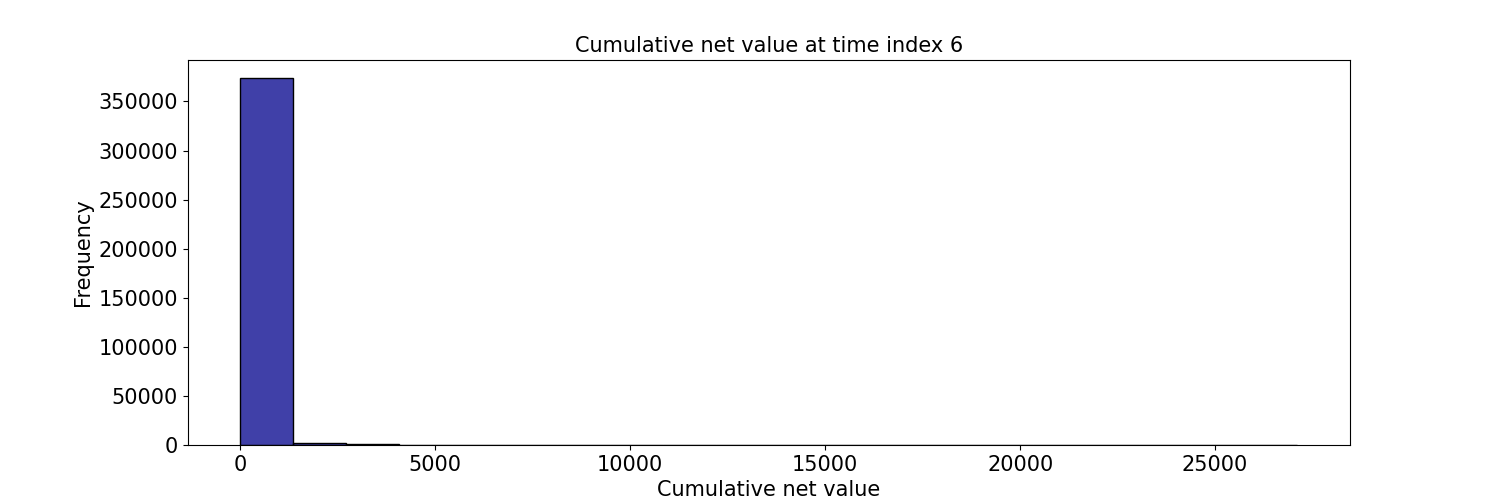
\includegraphics[height=1.8in]{cumulative_net_time_index_6}
  \caption{Distirbution of target variable : Net GMV}
  \label{fig:histogram_net_gmv}
\end{figure}

As discussed earlier, the Conditional Average Treatment Effect (\gls{CATE}) is simply the estimation of the Average Treatment Effect (\gls{ATE}) within groups defined by covariates. These covariates dictate the dimensional space 
in which the heterogeneity of the causal effect will be observed. They were created based on business knowledge, considering characteristics that could potentially correlate with the causal effect on the target metric (net GMV).

Extensive data manipulation was performed to construct a pool of variables and the table below describes all constructed variables along with a brief description.


\begin{table}[ht]
  \caption{Description of constructed variables.}
  \label{tab:variables}
\centering
\begin{adjustbox}{max width=\textwidth}
\begin{tabular}{ll}
  \toprule
  \textbf{Feature} & \textbf{Description} \\
  \midrule
  $count\_total\_concluded\_orders\_last\_91d$ & Total concluded orders in the last 91 days \\
  $count\_total\_concluded\_orders\_lifetime$ & Total concluded orders in lifetime \\
  $count\_total\_concluded\_orders\_last\_month$ & Total concluded orders in the last month \\
  $count\_food\_delivery\_concluded\_orders\_last\_91d$ & Total food delivery concluded orders in the last 91 days \\
  $count\_food\_delivery\_concluded\_orders\_lifetime$ & Total food delivery concluded orders in lifetime \\
  $count\_food\_delivery\_concluded\_orders\_last\_month$ & Total food delivery concluded orders in the last month \\
  $count\_food\_delivery\_dawn\_concluded\_orders\_last\_91d$ & Total food delivery dawn concluded orders in the last 91 days \\
  $count\_food\_delivery\_dawn\_concluded\_orders\_lifetime$ & Total food delivery dawn concluded orders in lifetime \\
  $count\_food\_delivery\_dawn\_concluded\_orders\_last\_month$ & Total food delivery dawn concluded orders in the last month \\
  $count\_food\_delivery\_breakfast\_concluded\_orders\_last\_91d$ & Total food delivery breakfast concluded orders in the last 91 days \\
  $count\_food\_delivery\_breakfast\_concluded\_orders\_lifetime$ & Total food delivery breakfast concluded orders in lifetime \\
  $count\_food\_delivery\_lunch\_concluded\_orders\_last\_91d$ & Total food delivery lunch concluded orders in the last 91 days \\
  $count\_food\_delivery\_lunch\_concluded\_orders\_lifetime$ & Total food delivery lunch concluded orders in lifetime \\
  $count\_food\_delivery\_lunch\_concluded\_orders\_last\_month$ & Total food delivery lunch concluded orders in the last month \\
  $count\_food\_delivery\_snack\_concluded\_orders\_last\_91d$ & Total food delivery snack concluded orders in the last 91 days \\
  $count\_food\_delivery\_snack\_concluded\_orders\_lifetime$ & Total food delivery snack concluded orders in lifetime \\
  $count\_food\_delivery\_snack\_concluded\_orders\_last\_month$ & Total food delivery snack concluded orders in the last month \\
  $count\_food\_delivery\_dinner\_concluded\_orders\_last\_91d$ & Total food delivery dinner concluded orders in the last 91 days \\
  $count\_food\_delivery\_dinner\_concluded\_orders\_lifetime$ & Total food delivery dinner concluded orders in lifetime \\
  $count\_food\_delivery\_dinner\_concluded\_orders\_last\_month$ & Total food delivery dinner concluded orders in the last month \\
  $sum\_total\_concluded\_orders\_paid\_amount\_last\_91d$ & Sum of total concluded orders paid amount in the last 91 days \\
  $sum\_total\_concluded\_orders\_paid\_amount\_lifetime$ & Sum of total concluded orders paid amount in lifetime \\
  $sum\_food\_delivery\_concluded\_orders\_paid\_amount\_last\_91d$ & Sum of food delivery concluded orders paid amount in the last 91 days \\
  $sum\_food\_delivery\_concluded\_orders\_paid\_amount\_lifetime$ & Sum of food delivery concluded orders paid amount in lifetime \\
  $sum\_food\_delivery\_dawn\_concluded\_orders\_paid\_amount\_last\_91d$ & Sum of food delivery dawn concluded orders paid amount in the last 91 days \\
  $sum\_food\_delivery\_dawn\_concluded\_orders\_paid\_amount\_lifetime$ & Sum of food delivery dawn concluded orders paid amount in lifetime \\
  $sum\_food\_delivery\_breakfast\_concluded\_orders\_paid\_amount\_last\_91d$ & Sum of food delivery breakfast concluded orders paid amount in the last 91 days \\
  $sum\_food\_delivery\_breakfast\_concluded\_orders\_paid\_amount\_lifetime$ & Sum of food delivery breakfast concluded orders paid amount in lifetime \\
  $sum\_food\_delivery\_lunch\_concluded\_orders\_paid\_amount\_last\_91d$ & Sum of food delivery lunch concluded orders paid amount in the last 91 days \\
  $sum\_food\_delivery\_lunch\_concluded\_orders\_paid\_amount\_lifetime$ & Sum of food delivery lunch concluded orders paid amount in lifetime \\
  $sum\_food\_delivery\_snack\_concluded\_orders\_paid\_amount\_last\_91d$ & Sum of food delivery snack concluded orders paid amount in the last 91 days \\
  $sum\_food\_delivery\_snack\_concluded\_orders\_paid\_amount\_lifetime$ & Sum of food delivery snack concluded orders paid amount in lifetime \\
  $sum\_food\_delivery\_dinner\_concluded\_orders\_paid\_amount\_last\_91d$ & Sum of food delivery dinner concluded orders paid amount in the last 91 days \\
  $sum\_food\_delivery\_dinner\_concluded\_orders\_paid\_amount\_lifetime$ & Sum of food delivery dinner concluded orders paid amount in lifetime \\
  $count\_cancelled\_orders\_last\_365d$ & Total cancelled orders in the last 365 days \\
  $count\_cancelled\_orders\_lifetime$ & Total cancelled orders in lifetime \\
  $count\_food\_delivery\_cancelled\_orders\_last\_365d$ & Total food delivery cancelled orders in the last 365 days \\
  $count\_food\_delivery\_cancelled\_orders\_lifetime$ & Total food delivery cancelled orders in lifetime \\
  $count\_food\_delivery\_dawn\_cancelled\_orders\_last\_365d$ & Total food delivery dawn cancelled orders in the last 365 days \\
  $count\_food\_delivery\_dawn\_cancelled\_orders\_lifetime$ & Total food delivery dawn cancelled orders in lifetime \\
  $count\_food\_delivery\_breakfast\_cancelled\_orders\_lifetime$ & Total food delivery breakfast cancelled orders in lifetime \\
  $count\_food\_delivery\_lunch\_cancelled\_orders\_last\_365d$ & Total food delivery lunch cancelled orders in the last 365 days \\
  $count\_food\_delivery\_lunch\_cancelled\_orders\_lifetime$ & Total food delivery lunch cancelled orders in lifetime \\
  $count\_food\_delivery\_snack\_cancelled\_orders\_last\_365d$ & Total food delivery snack cancelled orders in the last 365 days \\
  $count\_food\_delivery\_snack\_cancelled\_orders\_lifetime$ & Total food delivery snack cancelled orders in lifetime \\
  $count\_food\_delivery\_dinner\_cancelled\_orders\_last\_365d$ & Total food delivery dinner cancelled orders in the last 365 days \\
  $count\_food\_delivery\_dinner\_cancelled\_orders\_lifetime$ & Total food delivery dinner cancelled orders in lifetime \\
  $count\_groceries\_concluded\_orders\_last\_91d$ & Total groceries concluded orders in the last 91 days \\
  $count\_groceries\_concluded\_orders\_lifetime$ & Total groceries concluded orders in lifetime \\
  $count\_groceries\_market\_concluded\_orders\_last\_91d$ & Total groceries market concluded orders in the last 91 days \\
  $count\_groceries\_market\_concluded\_orders\_lifetime$ & Total groceries market concluded orders in lifetime \\
  $count\_groceries\_pharma\_concluded\_orders\_lifetime$ & Total groceries pharma concluded orders in lifetime \\
  $count\_groceries\_pet\_concluded\_orders\_lifetime$ & Total groceries pet concluded orders in lifetime \\
  $count\_groceries\_beverage\_concluded\_orders\_lifetime$ & Total groceries beverage concluded orders in lifetime \\
  $count\_groceries\_dark\_store\_concluded\_orders\_lifetime$ & Total groceries dark store concluded orders in lifetime \\
  $sum\_groceries\_concluded\_orders\_paid\_amount\_last\_91d$ & Sum of groceries concluded orders paid amount in the last 91 days \\
  $sum\_groceries\_concluded\_orders\_paid\_amount\_lifetime$ & Sum of groceries concluded orders paid amount in lifetime \\
  $sum\_groceries\_market\_concluded\_orders\_paid\_amount\_last\_91d$ & Sum of groceries market concluded orders paid amount in the last 91 days \\
  $sum\_groceries\_market\_concluded\_orders\_paid\_amount\_lifetime$ & Sum of groceries market concluded orders paid amount in lifetime \\
  $sum\_groceries\_pharma\_concluded\_orders\_paid\_amount\_last\_91d$ & Sum of groceries pharma concluded orders paid amount in the last 91 days \\
  $sum\_groceries\_pharma\_concluded\_orders\_paid\_amount\_lifetime$ & Sum of groceries pharma concluded orders paid amount in lifetime \\
  $sum\_groceries\_pet\_concluded\_orders\_paid\_amount\_last\_91d$ & Sum of groceries pet concluded orders paid amount in the last 91 days \\
  $sum\_groceries\_pet\_concluded\_orders\_paid\_amount\_lifetime$ & Sum of groceries pet concluded orders paid amount in lifetime \\
  $sum\_groceries\_beverage\_concluded\_orders\_paid\_amount\_last\_91d$ & Sum of groceries beverage concluded orders paid amount in the last 91 days \\
  $sum\_groceries\_beverage\_concluded\_orders\_paid\_amount\_lifetime$ & Sum of groceries beverage concluded orders paid amount in lifetime \\
  $sum\_groceries\_dark\_store\_concluded\_orders\_paid\_amount\_last\_91d$ & Sum of groceries dark store concluded orders paid amount in the last 91 days \\
  $sum\_groceries\_dark\_store\_concluded\_orders\_paid\_amount\_lifetime$ & Sum of groceries dark store concluded orders paid amount in lifetime \\
  $count\_groceries\_cancelled\_orders\_last\_365d$ & Total groceries cancelled orders in the last 365 days \\
  $count\_groceries\_cancelled\_orders\_lifetime$ & Total groceries cancelled orders in lifetime \\
  $count\_groceries\_market\_cancelled\_orders\_lifetime$ & Total groceries market cancelled orders in lifetime \\
  $count\_groceries\_beverage\_cancelled\_orders\_lifetime$ & Total groceries beverage cancelled orders in lifetime \\
  $sum\_shopping\_concluded\_orders\_paid\_amount\_last\_91d$ & Sum of shopping concluded orders paid amount in the last 91 days \\
  $sum\_shopping\_concluded\_orders\_paid\_amount\_lifetime$ & Sum of shopping concluded orders paid amount in lifetime \\
  $sessions\_m1$ & Number of sessions in the last month \\
  $converted\_sessions\_m1$ & Number of converted sessions in the last month \\
  $days\_with\_sessions\_m1$ & Number of days with sessions in the last month \\
  $net\_revenue\_m1$ & Net revenue in the last month \\
  $direct\_costs\_m1$ & Direct costs in the last month \\
  $indirect\_costs\_m1$ & Indirect costs in the last month \\
  $operation\_margin\_m1$ & Operation margin in the last month \\
  $avg\_restaurants\_available\_m1$ & Average number of restaurants available in the last month \\
  $avg\_centroid\_income\_m1$ & Average centroid income in the last month \\
  \bottomrule
\end{tabular}
\end{adjustbox}
\end{table}

Those features contain information about the user's behavior, such as the number of orders, the total amount spent, the number of sessions, revenue generated among different time windows, such
as the last month, the last 91 days, and the lifetime. The features also include information about the user's location, such as the average income of the user's location, and the average number of restaurants
available in the user's favorite location.

The mantra "garbage in, garbage out" also applies to uplift modeling. Therefore, a rigorous feature selection process must be conducted. This and other steps included in the iterative modeling process will be presented in the next chapter.